% !TeX root = ./point_v_continuum.tex
\documentclass[letterpaper, 10pt]{article}
\usepackage[margin=0.75in]{geometry}
\usepackage{microtype}
\usepackage{graphicx}
\usepackage{mathpazo}
\usepackage{amsmath}
\usepackage{setspace}
\onehalfspacing

\begin{document}
\section*{Point Estimate vs Continuum Estimates}
Thus far in the project, Nathan and I have been going about the estimates by
choosing a particular growth rate $\lambda$ (typically $\lambda = 0.5\,
\text{hr}^{-1}$, $t_\text{double} = 5000 \,\text{s}$) and using some
rules-of-thumb to compute how many protein complexes involved in a given
biological process should be present. In general, this approach has worked well
and our estimates have landed in the ball park of the observed copy numbers,
ultimately allowing us to proclaim that we know what "sets the scale".

However, I (Griffin) have been trying to abstract these point estimates to a
continuum of growth rates ($\lambda \in [0, 2]\, \text{hr}^{-1}$). My reasoning
for doing so is primarily due to some comments we received during Manu's group
meeting as well as comments I received from friends who have said "shouldn't you
be predicting the slope?" Furthermore, I (Griffin) think one can make the
argument that there are \textit{two} scales that we must be able to
quantitatively define in order to "understand" the process. The first scale is
the absolute copy numbers of the complexes (like we have done for the point
estimates). The second scale is the dependence on the growth rate. In many
cases, I believe this boils down to either a dependence on the cell volume (or
cell size, depending on your favorite nomenclature) \textit{or} a dependence on
the chromosome copy number. These two "natural variables" have both qualitative
and quantitative differences. 

As an example, let's walk through an estimate using both the point estimate and
the continuum estimate approaches. While we can do this for any process, I've
chosen to consider the dynamics of phosphate transporters.

\section{Phosphate Transporters -- Background}
Phosphorus is critical to the cellular energy economy in the form of
high-energy phosphodiester bonds making up DNA, RNA, and the NTP energy pool
as well as playing a critical role in the post-translational modification of
proteins and defining the polar-heads of lipids. In total, phosphorus makes
up $\approx$3\% of the cellular dry mass which in typical experimental
conditions is in the form of inorganic phosphate. The cell membrane has
remarkably low permeability to this highly-charged and critical molecule,
therefore requiring the expression of active transport systems. In \textit{E. coli}, the proton electrochemical gradient across the inner membrane is
leveraged to transport inorganic phosphate into the cell
\cite{rosenberg1977}. Proton-solute symporters are widespread in \textit{E.
coli} \cite{ramos1977, booth1979} and can have rapid transport rates of 50
molecules per second for sugars and other solutes (BNID: 103159; 111777,
\cite{milo2010}). Proton transporters, such as those in the F$_1$-F$_0$ ATP
synthase, leverage the proton chemical gradient
to drive conformational changes in the protein complex and can shuttle $\approx
1000$ protons per second (BNID: 104890; 103390, \cite{milo2010}). 
In \textit{E. coli} the PitA phosphate transport system has
been shown to be very tightly coupled with the proton electrochemical gradient
with a 1:1 proton:phosphate stoichiometric ratio \cite{harris2001,
feist2007}. While the precise rate per transporter is not well known for the
\textit{E. coli} Pit system, we can state that it is likely in between the
aforementioned rates for sugar transport and ATP synthesis, on the order of
$\approx$ 300 phosphates transported per second. 

\subsection{Point Estimate}
Using the fact that the cellular dry mass is $\approx 3\%$ phosphorus and
transport through the Pit system of \textit{E. coli} is $\approx 300$ phosphates
per second, we can immediately compute a point estimate for the number of
transporters present per cell.

We begin with considering a modest \textit{E. coli} doubling time of $\approx
5000 \text{s}$. At this growth rate, we can approximate the cell as having a
total volume of $\approx 1\, \text{fL}$ which corresponds to a mass of $\approx
1\, \text{pg}$. Assuming that $\approx 70\%$ of the \textit{E. coli} cell mass
is water, and $\approx 3\%$ of the dry mass is phosphorus, we arrive at total
phosphorus mass fraction of 
\begin{equation}
    \theta_\text{P} \approx 0.3 \times 0.03 \approx 0.01.
\end{equation}
Given that the molecular weight of
phosphorus is $30\,\text{Da}$, the total number of phosphorus atoms per cell can
be calculated as 
\begin{equation}
N_\text{phosphorus} \approx \frac{\theta_\text{P} \times 1\,\text{pg}}{30\,\text{Da}}\times \frac{6\times10^{11}\,\text{Da}}{1\,\text{pg}} \approx 2 \times 10^8\, \text{P}.
\end{equation}

We can now assume that all phosphorus atoms enter the cell via phosphate and
make the further approximation that this transport comes exclusively through the
Pit system. Using our estimate of $\approx 300$ phosphates per second as the
transport rate via the Pit system transporters, we arrive at an estimate for the
total number of transporters to be 
\begin{equation}
    N_\text{transporters} \approx \frac{2 \times 10^8\,\text{P}}{1\,\text{cell}}\times \frac{1\,\text{s}\cdot\text{transporter}}{300\,\text{phosphate}}\frac{1\,\text{cell}}{5000\,\text{s}}\approx 150\, \text{transporters}.
    \label{eq:point_estimate}
\end{equation}

Figure \ref{fig:point_estimate} shows a comparison of this estimate the
experimentally measured values. While our estimate is very much in line with
the observed numbers, we emphasize that this is likely a slight over estimate
of the number of transporters needed as there are other phosphorous
scavenging systems, such as the ATP-dependent phosphate transporter Pst
system which we have neglected.

\begin{figure}
    \centering{
        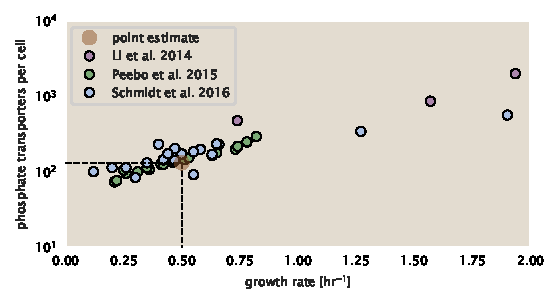
\includegraphics{../../figures/phosphate_point_estimate.pdf}
        \caption{\textbf{Point estimate for the number of phosphate
        transporters and comparison with data.} Point estimate as outlined in
        Eq. \ref{eq:point_estimate} is shown in brown. Experimental
        meausrements of the total number of PitA and PitB phosphate
        transporters for each data set are shown as colored points. Vertical
        dashed line indicates a doubling time of 5000 seconds and horizontal
        dashed line indicates a copy number of $\approx 150$ per cell.}
        \label{fig:point_estimate}
    }
\end{figure}


\subsection{Continuum Estimate}
Rather than choosing an arbitrary doubling time and rule-of-thumb for the cell
mass, we can draw upon the detailed literature of \textit{E. coli} growth to
estimate the number of transporters needed across a continuum of growth rates,
assuming that the entirety of the transported phosphate ions are used in the
generation of new cell mass or energy production. 

Recent single-cell measurements have extensively characterized the
time-dependent growth of \textit{E. coli} in terms of dimensions, cell mass, and
cell volume. A combination of recent works by Fangwei Si \textit{et al.}
\cite{si2017, si2019} have revealed that cell volume $V$ is exponential with
growth rate $\lambda$ and follows an approximate scaling of 
\begin{equation}
    V(\lambda) \approx ae^{b\lambda},
    \label{eq:si_vol}
\end{equation}
where $a \approx 0.5\,\mu\text{m}^3$ and $b\approx 1\,\text{hr}$. Using this expression, a growth-rate independent buoyant density of
$\rho \approx 1.1 \,\text{pg} / \mu\text{m}^3$ (BNID: 103875, \cite{milo2010}), a
growth-rate independent elemental composition of $\theta_P \approx 0.01$ of the
total cell mass, and the atomic weight $m_P = 30 Da$, the
total number of phosphorus atoms needed as a function of growth rate
$N_\text{P}(\lambda)$ can be
computed as 
\begin{equation}
    N_\text{P}(\lambda) \approx \frac{\theta_\text{P}\rho V(\lambda)}{m_{P}}.
\end{equation}

Assuming that the rate of phosphate transport $r = 300\,\text{PO}_4^{2-} \cdot s^{-1} \cdot \text{transporter}$ is independent of
the growth rate, we can now compute the estimated number of transporters per
cell as a function of growth rate as 
\begin{equation}
N_\text{transporters}  \approx \frac{\theta_\text{P}\rho V(\lambda)}{m_\text{P}r\left(\frac{\log 2}{\lambda}\right)},
\label{eq:continuum_estimate}
\end{equation}
where the factor $\log{2} / \lambda$ computes the doubling time $t_\text{double}$
\begin{equation}
    t_\text{double} = \log{2} / \lambda.
\end{equation}
Figure \ref{fig:continuum_estimate} shows the result of Eq.
\ref{eq:continuum_estimate} plotted as a function of the growth rate and
compares it with the experimental measurements. Overall, we find that this
simple estimate based on cell scaling is sufficient to describe both the
absolute number of the phosphate transporters as well as the dependence on the
growth rate. We note that this simple scaling argument significantly
underestimates the number of phosphate transporters at very slow growth rates
($\lambda < 0.2\,\text{hr}^{-1}$). This may be due to the fact that at very slow
growth rates, the cellular physiology prioritizes other metabolic functions over
he generation of new cell mass (to anthropomorphize, the cell focuses on
survival rather then reproduction). 

\begin{figure}
    \centering{
        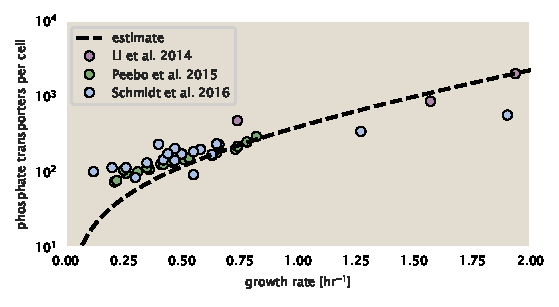
\includegraphics{../../figures/phosphate_continuum_estimate.pdf}
        \caption{\textbf{Estimated number of phosphate tranposrters needed as
        a function of growth rate.} Dashed line shows the predicted scaling as
        prescribed by Eq. \ref{eq:continuum_estimate}. Colored points correspond
        to the total number of PitA and PitB transporters present in each
        dataset.}
        \label{fig:continuum_estimate}
    }
\end{figure}

\subsection{Generalization to Other Transport Processes}
The scaling argument given in Eq. \ref{eq:continuum_estimate} can be cast in
very general terms for an array of transported materials. For element $X$ the
number of transporters can be computed as 
\begin{equation}
N_\text{X} \approx \frac{\theta_\text{X}\rho V(\lambda)}{m_\text{X}r_\text{X}\left(\frac{\log 2}{\lambda}\right)},
\end{equation}
where the rate $r_\text{X}$ must be in units of atoms per unit time. Figure
\ref{fig:continuum_tport} shows this approach applied to glucose, phosphorus,
and sulfur transport. 

\begin{figure}
    \centering{
        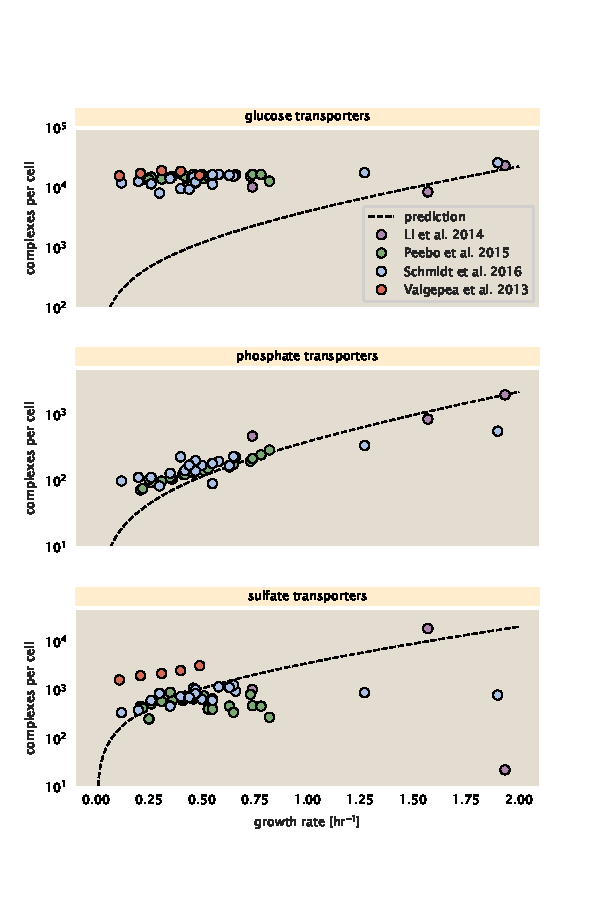
\includegraphics{../../figures/tport_system_scaling.pdf}
        \caption{\textbf{Growth-rate dependent scaling of transport systems.} The estimated growth rate dependence for the transport of glucose, phosphorus, and sulfate is shown as dashed lines from top to bottom, respectively. Experimental measurements are shown as colored points.}
        \label{fig:continuum_tport}
    }
\end{figure}


\section{Arguments and Compromise}
Nathan and I have been discussing this for quite some time and I think we each
have mid-grade level chilis about which way to proceed. I am in favor of the
continuum estimate approach and Nathan is partial to using only the point
estimates. 

Here’s my paraphrased version of Nathan’s argument (with Nathan’s approval) for
using the point estimate only:
\begin{enumerate}
\item We want to provide some rationale just for the observed scale, and not necessarily the dependence. We consider the dependence for translation as we know some more details about how the parameters change.
\item It’s not fair to make predictions at very slow growth rates because we only consider the processes necessary to make new cell mass. At slow growth rates, maybe this isn’t totally fair.
\item The scaling will look the same (qualitatively) for every category where the cell size / cell mass is the natural variable.
\item Adding the exponential scaling for cell volume is very \textit{E. coli} specific and undercuts the “fundamental limits for bacterial division” which is the main point of the paper.
\end{enumerate}

Here’s my argument for estimating across all growth rates.
\begin{enumerate}
\item While some of these parameters may change (i.e. transport rates), our rules-of-thumb for \textit{E. coli} come from different growth regimes. We implicitly make the assumption that the rate of transport (for example) is growth rate independent.
\item The process for drawing predictions across growth rates is the exact same as using a standard time of 5000 s, just using different starting values for the cell mass and division time.
\item Maybe we can’t say much at exceedingly slow growth rates, but most of the \textit{E. coli} specific data we are comparing to lies in the regime of “moderate” growth rates and is probably fair to consider in this manner. A way around this is maybe to not show the scaling below ~ 0.1 hr$^{-1}$?
\item The processes we consider in the paper can be thought of as fundamental
limits, but all of our estimates and arguments do ultimately come from \textit{E. coli}
specific biology. For example, we aren’t saying anything about extracellular
electron transport which ends up being a critical mode of respiration for a lot
of non \textit{E. coli} flavored bugs.
\end{enumerate}


One compromise is that we proceed with the point estimates as we have currently
been doing for the main text and have the continuum approach for each case in
the SI. For the main-text figures, we can include both, an example of which is
shown in Fig. \ref{fig:compromise}

\begin{figure}
    \centering{
        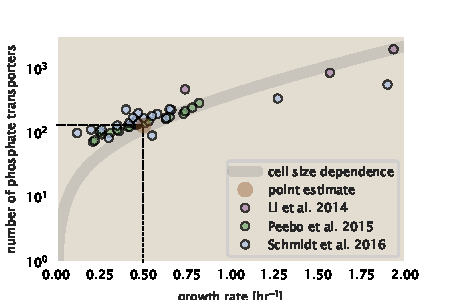
\includegraphics{../../figures/phospho_tport_scaling_plot.pdf}
        \caption{\textbf{An example of a compromise plot showing both the point
        estimate and the cell-size scaling argument.} This shows what the
        phosphate transporter plot for the main-text would look like under a
        compromise where the focus is still on the point estimate, but we also
        include the predicted scaling with growth rate and direct the reader to
        the SI for more information.}
        \label{fig:compromise}
    }
\end{figure}

\bibliographystyle{unsrt}
\bibliography{../manuscript/library.bib}
\end{document}